\documentclass[10pt,twocolumn,letterpaper]{article}

\usepackage{wacv}
\usepackage{times}
\usepackage{epsfig}
\usepackage{amsmath}
\usepackage{amssymb}
\usepackage{graphicx}
\usepackage[font=small]{caption}
\usepackage{subcaption}
\captionsetup{compatibility=false}
\usepackage{color}
\usepackage{url}
\usepackage{comment}
\usepackage{multirow}
\usepackage{tabularx}
\newcolumntype{Y}{>{\centering\arraybackslash}X}
% Include other packages here, before hyperref.

% If you comment hyperref and then uncomment it, you should delete
% egpaper.aux before re-running latex.  (Or just hit 'q' on the first latex
% run, let it finish, and you should be clear).
\usepackage[pagebackref=true,breaklinks=true,letterpaper=true,colorlinks,bookmarks=false]{hyperref}

%\wacvfinalcopy % *** Uncomment this line for the final submission

\def\wacvPaperID{****} % *** Enter the wacv Paper ID here
\def\httilde{\mbox{\tt\raisebox{-.5ex}{\symbol{126}}}}

% Pages are numbered in submission mode, and unnumbered in camera-ready
\ifwacvfinal\pagestyle{empty}\fi
\begin{document}
\title{A Motion Blur Resilient Fiducial Marker For Quadcopter Imaging}
\maketitle

\begin{abstract}
This paper describes the design and evaluation of a binary fiducial marker
for use with low-cost quadcopters.  Fiducial markers are commonly placed
in environments to provide a uniquely identifiable object in the scene.
For quadcopter applications, fiducials are often used for evaluating planning
algorithms by allowing ground truth positions in the scene to be detected from
the quadcopter's camera. Quadcopters, however, are subject to quick and
unstable motions that can cause significant motion blur that severely affects
the detection rate of existing fiducial markers. This problem motivated us to
design a fiducial that is robust to motion blur. Our proposed fiducial design
uses concentric circles with the observation that the direction perpendicular
to the motion blur direction will be relatively unaffected by the blur. This
allows the fiducial code along the blur direction to be recognized.
The circular design allows this to work for all motion blur directions. We
detail the design and detection algorithm for our fiducial and show that our
marker can significantly outperform existing fiducial markers in scenes
captured with a quadcopter.
\end{abstract}

\section{Introduction}

The recent availability of low-cost quadcopters have helped to fuel significant
efforts in research focused on unmanned aerial vehicles. Navigation and planning of
these vehicles is typically performed using onboard inertial sensors and/or
vision based modules that uses visual cues in the real world~(e.g.,
\cite{Davison:2007,Engel12,Engel13}). However, to evaluate the effectiveness of
navigation methods, fiducial markers are commonly placed into the environment
to provide additional information that serves for ground-truth positional
measurements (e.g., \cite{Bosnak:2012,Lim09,Klopschitz:2007}).

In order to be effective, fiducial markers (or simply, fiducials) need
to be easily detected in the scene. A variety of fiducial markers
have been proposed in the literature
(e.g.,~\cite{NaimarkF02,ARToolkit02,Fiala05,Pitag13,runetag11}).
These take the form of binary codes arranged into rectangular grids (\cite{ARToolkit02,Fiala05})
or other geometric primitives arranged in predefined spatial patterns
(\cite{NaimarkF02,Pitag13,runetag11}).
Figure \ref{fig:teaser}-(a) shows the popular ARTag \cite{Fiala05} as
seen from a quadcopter. A problem for existing fiducials is that low-cost quadcopters
often exhibit very quick and erratic physical movements that
result in motion blur in the quadcopter's onboard camera. This motion blur has
an adverse effect on the recognition of fiducial markers. This can be seen in
Figure \ref{fig:teaser}-(b) where the ARTag cannot be recognized due to motion
blur. This is not too surprising as most existing fiducials are not
designed to handle motion blur.

Compounding this problem is the additional issue of dropped video frames from
the quadcopter's wireless communication module. This means that not only is
blur a problem, but there may be large discontinuities in the pattern's
position due to missing video frames. As we will show in Section 4, this later problem
makes it challenging to apply tracking algorithms that can exploit temporal
coherence for determining the fiducial's position.

\noindent\textbf{Contribution}~~To address these problems, we propose a
fiducial that is designed to be resistant to motion blur. Our design is based on
concentric circles as shown in Figure \ref{fig:teaser}-(c,d). The design is based
on the observation that motion blur from a quadcopter tends to be linear in
nature. As such, when our code is blurred, there is no blur in the direction
perpendicular to the direction of motion.  This allows the signature of the
fiducial to remain intact in any direction. In addition, by using concentric
rings, we can treat the presence or absence of a ring as a bit, allowing us to
assign a code to the marker. Our experiments show that this design can
significantly outperform existing codes in the presence of motion blur. As far
as we are aware, this is the first work to propose a blur resistant marker.

The remainder of this paper is organized as follows.  Section 2 gives an
overview of related work related to fiducials as well as the related problem of
tracking. Section 3 discusses our design and detection algorithm as well as
the performance of existing codes under motion blur. Section 4 shows several
experiments using quadcopter imagery. This is followed by a discussion and
summary in Section 5 and 6 respectively.

\begin{figure}
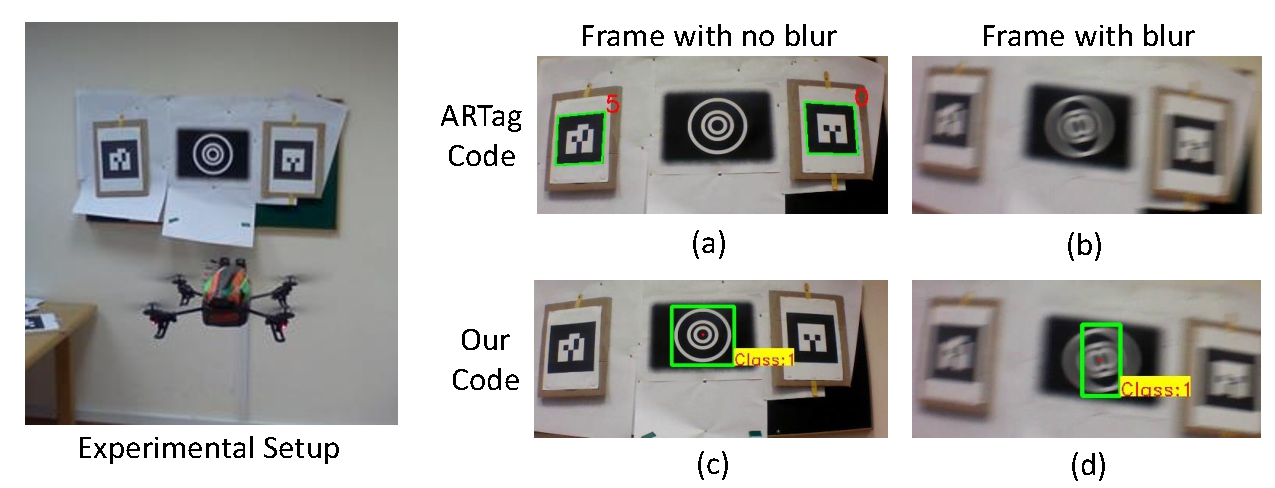
\includegraphics[width=\linewidth]{teaser.pdf}
\caption{This figure shows the experimental setup and comparison of
output of ALVAR~\cite{alvar} (for detecting ARTag) versus our blur resistant
fiducial in a normal and blurred video frame. The scene contains two ARTags and our code.
(a) shows that the ARTag can be detected when the image has no blur.
(b) shows that ARTags are no longer detectable due to the blur.
(c-d) show the same images in (a) and (b) where our code is being detected.}
\label{fig:teaser}
\end{figure}

\section{Related Work}

Our work is related to two areas: fiducial markers and object tracking. We
briefly discuss work done in both areas.

\begin{figure}
\centering
 \begin{subfigure}[b]{0.19\textwidth}
  \centering
  
\includegraphics[width=0.8\linewidth]{intersense.jpg}
  Circular Data Matrix~\cite{NaimarkF02}
 \end{subfigure}\quad
 \begin{subfigure}[b]{0.14\textwidth}
 \centering
  
\includegraphics[width=\linewidth]{pattKanji.pdf}
  ARToolkit~\cite{ARToolkit02}
 \end{subfigure}\quad
 \begin{subfigure}[b]{0.14\textwidth}
  \centering
  
\includegraphics[width=\linewidth]{ARtag.jpg}
  ARTag\quad~\cite{Fiala05}
 \end{subfigure}\quad
 \begin{subfigure}[b]{0.14\textwidth}
  \centering
  
\includegraphics[width=\linewidth]{pifiducial.jpg}
  PiTag\quad~\cite{Pitag13}
 \end{subfigure}\quad
 \begin{subfigure}[b]{0.14\textwidth}
  \centering
  
\includegraphics[width=\linewidth]{our_fiducial}
  Our Fiducial
 \end{subfigure}
 \caption{This figure shows the design of several existing fiducial markers.  While
 each code has their own pros and cons for various environments, none are
 designed to be recognized under motion blur.}
 \label{fig:previous_work}
\end{figure}

\noindent{\textbf{Fiducials}}~Figure~\ref{fig:previous_work} shows several
examples of existing fiducial markers.  Many designs use a two dimensional
barcode inside a rectangular grid. One example of such a fiducial is from the
ARToolkit~\cite{ARToolkit02}, a well known toolkit used in many augmented
reality (AR) applications. Kato and Billinghurst~\cite{kato-artoolkit}
demonstrated the use of ARToolkit to find the pose in video based AR
conferencing system.

Fiala~\cite{Fiala05} proposed a fiducial termed, ARTag, which is a
bi-tonal system consisting of a square border and an interior 6$\times$6 grid
of black or white cells. The improvement in ARTag compared to ARToolkit was
detection of corners instead of detection of lines to find possible pattern.
This proved to be more efficient than \cite{ARToolkit02} in terms of
recognition rate as well as the number of different patterns which can be
created.   The reliance on both line and corner detection hampers recognition
under motion blur.

There were also attempts to use circular patterns instead of rectangular.
Gatrell et al.~\cite{concentric} used concentric circles
for monocular pose estimation as well as object identification. Cho et al.
\cite{Cho:2001,Cho97fastcolor} have used multicolor rings instead of black and white rings~\cite{concentric} to increase possible number of fiducials.
These multicolor rings are used in wide area tracking in large scale
applications.  While based on a concentric rings, these approaches require
the full ring to be recognized which is not possible when the pattern undergoes directional
motion blur.

Naimark and Foxlin~\cite{NaimarkF02} proposed a circular bar code
called the Circular Data Matrix that is beneficial in terms of
easy detection and ability to have a large number
of uniquely identifiable codes.  To address the issue of occlusion,
Bergamasco et al.~\cite{runetag11} proposed the RUNE-tag fiducial by dividing
into number of circular dots arranged in circular fashion. RUNE-tags can be
detected even when up to 50\% of fiducial area is occluded. Bergamasco et
al.~\cite{Pitag13} proposed the PiTag fiducial, also composed of circular
structures but arranged in a rectangle to exploit projective invariant cross-ratio.
This provided similar occlusion resistance as RUNE-tag but with even less
circular dots. All of these techniques however rely on generic features
detection (e.g., circle detection) that break down under motion blur.

%Zhang et al.\cite{Zhang:2002} and Claus et al. \cite{ClausF04} have done
%quite comprehensive comparative study of various fiducial marker systems with
%respect to processing time, recognition rate and accuracy with
%respect to viewing angle and distance.

\noindent{\textbf{Tracking}}~~Fiducial detection between successive video
frames can be considered as a tracking problem where the tracked object is
fiducial itself.  There is a very large body of research dedicated to tracking and interested
readers are referred to~\cite{Yilmaz:2006} for a good survey.

Most tracking methods (e.g.,~\cite{Ross:2008,Wu:2009,Perez02,Mei:2009}) assume
the image sequence to be blur free. In reality, however, the presence of motion blur in 
a video sequence is often unavoidable. To this end, Wu et al.~\cite{Wu:2011}
proposed the Blur-driven Tracker (BLUT) framework for tracking motion-blurred targets. BLUT
is based on the observation that although motion blurs degrade the visual
features of the target, they at the same time, provide useful cues about the
movements to help tracking.

The BLUT framework successfully tracks blurred target when there is uniform motion
and the position of tracked object does not change drastically in successive
frames. But as we will demonstrate in Section 4, the erratic motion from quadcopters as
well as the problem of dropped video frames is beyond the current ability of such trackers.

\section{Design of Blur Resistant Fiducial}

We begin by first motivating the need for a new blur resistant fiducial by examining
the performance of prior fiducials under motion blur.  After this, we detail
our design as well as the detection algorithm used to find our marker in an image.

\subsection{Examining Prior Fiducials Under Motion Blur}\label{sec:blurtest}

Before we detail the design of our fiducial, we examine the performance of two
popular fiducials under motion blur.  Specifically we examine ARTags
~\cite{Fiala05} and PiTags~\cite{Pitag13} given their difference in geometry
design and the availability of API to develop applications to recognize the tags.
RUNE-tag~\cite{runetag11} currently does not provide access to the an
implementation to generate or recognize the tag.  The circular data
matrix~\cite{NaimarkF02} is available as a commercial product, however it
requires proprietary hardware to recognize the fiducial.

To evaluate the ARTag and PiTag under blur, we simulate the appearance of the
marker as seen by a quadcopter by scaling the tags to 150$\times$150 pixels.
Both fiducials are then blurred using linear motion blur at various
orientations with different blur scales. The blur motion ranged from 15 to 50
in magnitude (denoted in pixels), representing small to significant motion
blur. Figure \ref{fig:artag_pitag} shows the visual appearance of the blurred
tags. We then try to detect the markers using the ALVAR library~\cite{alvar} and
PiTag library~\cite{ros_pitag}. The table in the right side of
Figure~\ref{fig:artag_pitag} shows the recognition rate (in percentage) of two
fiducial markers at various blur scales over all the different orientations.
As we can see, the PiTag performance quickly diminishes under small amounts of
blur, while at 35 motion blur, the ARTag's recognition rate drops to less than
20\%.

\noindent\begin{minipage}[h!]{\textwidth}
\noindent\begin{minipage}{0.6\textwidth}
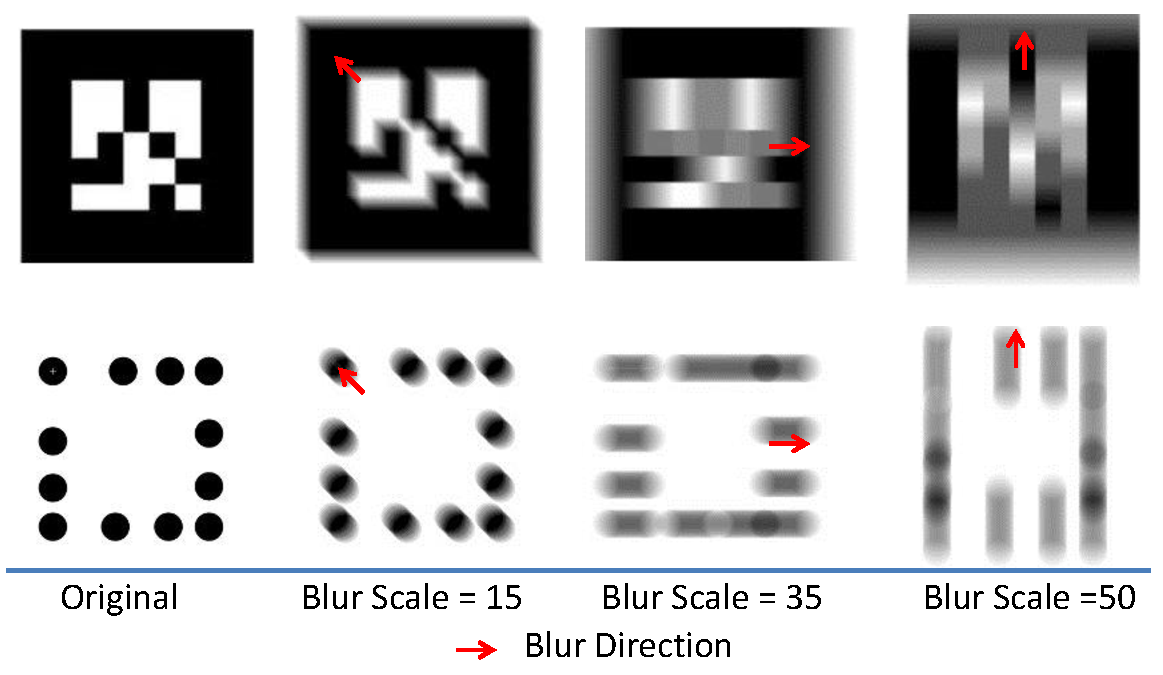
\includegraphics[width=\textwidth]{artag_pitag.pdf}
%\captionof{figure}{Blurred AR Tag and Pi--tag with various blur scales}
\end{minipage}
\begin{minipage}{0.35\textwidth}
%\captionof{table}{Recognition rate of AR Tag and Pi-tag fiducial marker atvarious blur scales}
\begin{tabularx}{\textwidth}{|Y|Y|Y|}
\cline{1-3}
\small{Blur} & \multicolumn{2}{c|}{ \small{Recognition Rate}}
\\\cline{2-3}
\small{Scale}& \small{PiTag} &	\small{ARTag} \\ \cline{1-3}
\small{15} & \small{100} & \small{100} \\ %\cline{1-3}
\small{30} & \small{0} & \small{100} \\  %\cline{1-3}
\small{35} & \small{0} & \small{19} \\ %\cline{1-3}
\small{50} & \small{0} & \small{0} \\ \cline{1-3}
\end{tabularx}
\end{minipage}
\captionof{figure}{Figure showing PiTag and ARTag blurred with various blur
scales at different orientations. Table on the right shows the recognition rate
(in percent) of both fiducial markers at various blur scales along all blur
orientations.  Recognition rates for both tags are significantly reduced due to
blur. For severe blur, detection is not possible.}
\label{fig:artag_pitag}
\end{minipage}

\subsection{Blur Resistant Fiducial}

We have designed a binary coded fiducial that uses concentric white rings of
equal widths on a black background with a blurred border\footnote{This design
can be inverted to have a white background with white rings.}. The
outermost and innermost rings represent the start and end of the code and is
embedded in the fiducial.  The binary code is represented by the presence (or
absence) of rings between ``marker'' rings.

\begin{figure}
\centering
  
\includegraphics[width=.18\linewidth]{newconcentric_00.pdf}
  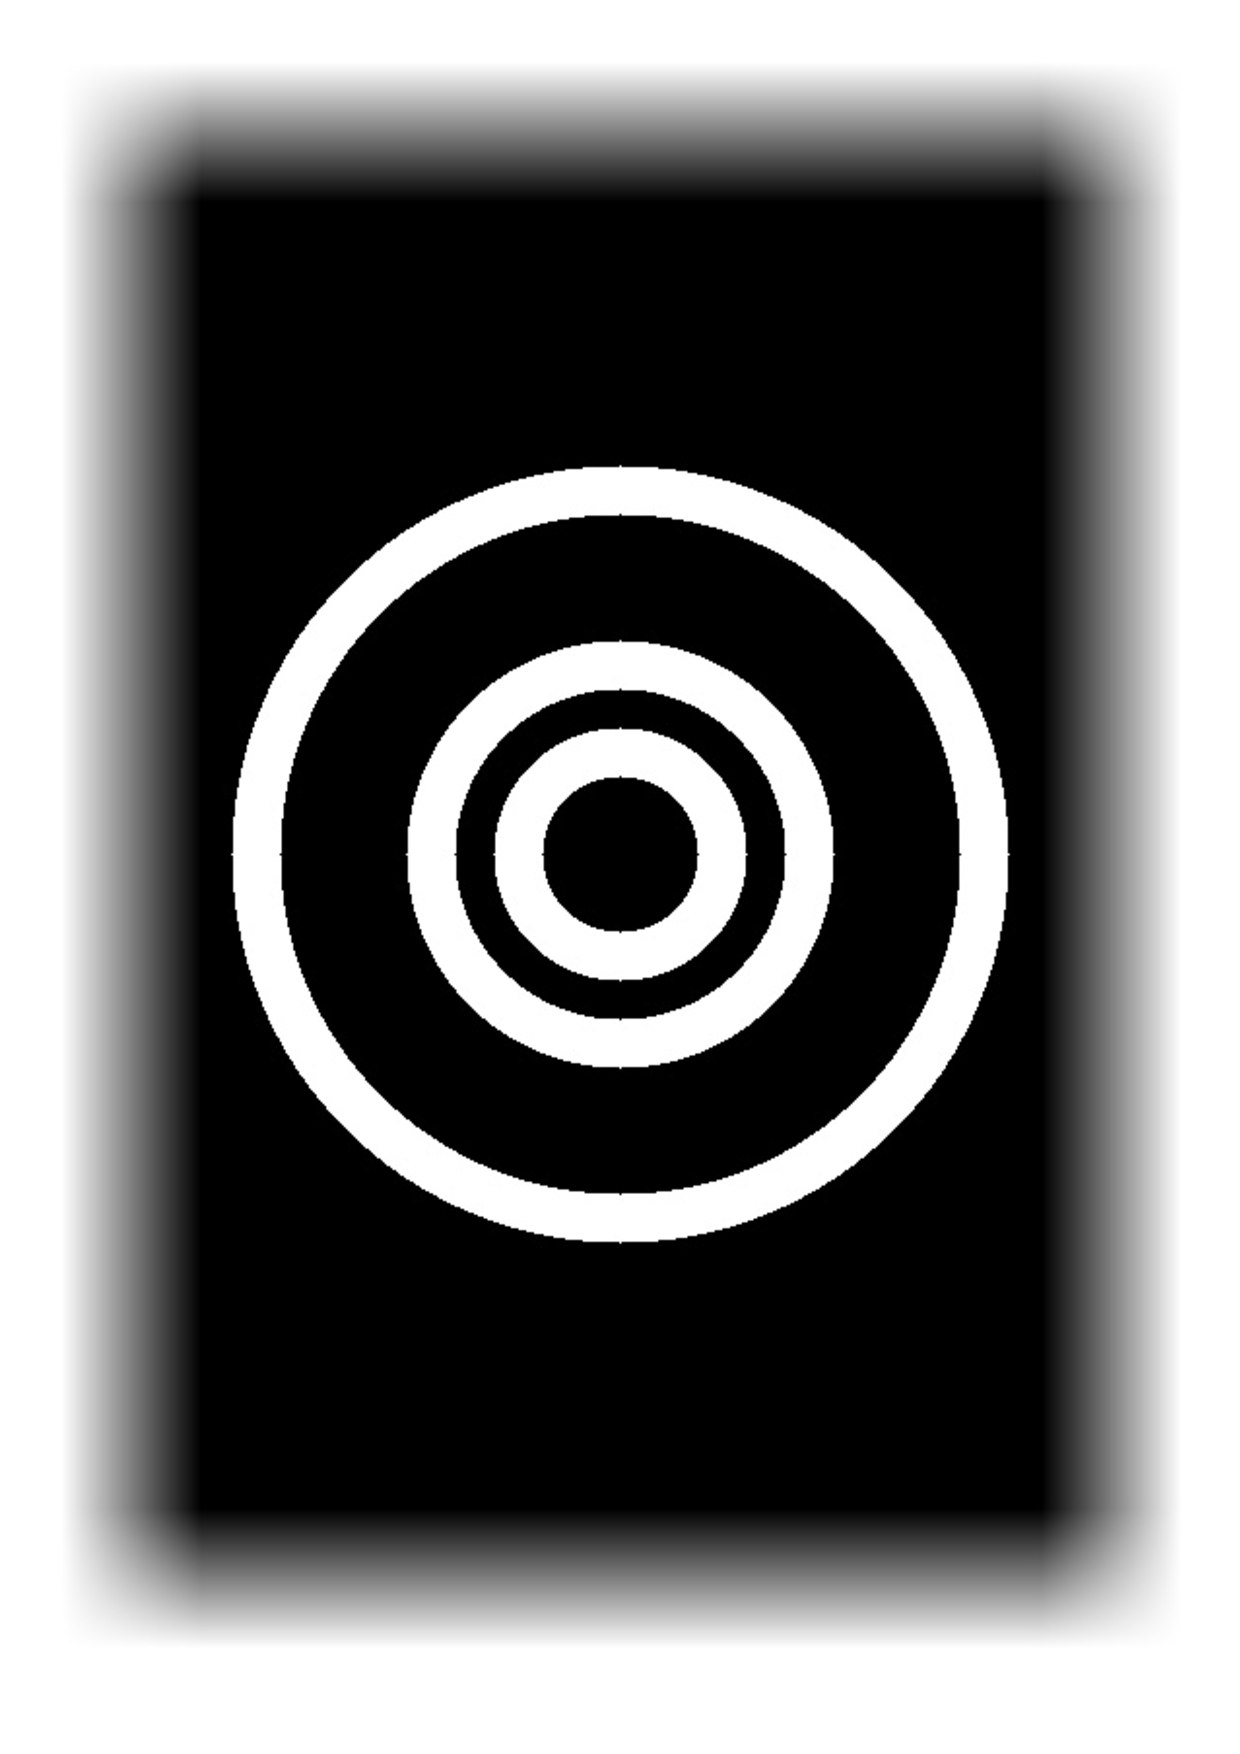
\includegraphics[width=.18\linewidth]{newconcentric_01.pdf}
  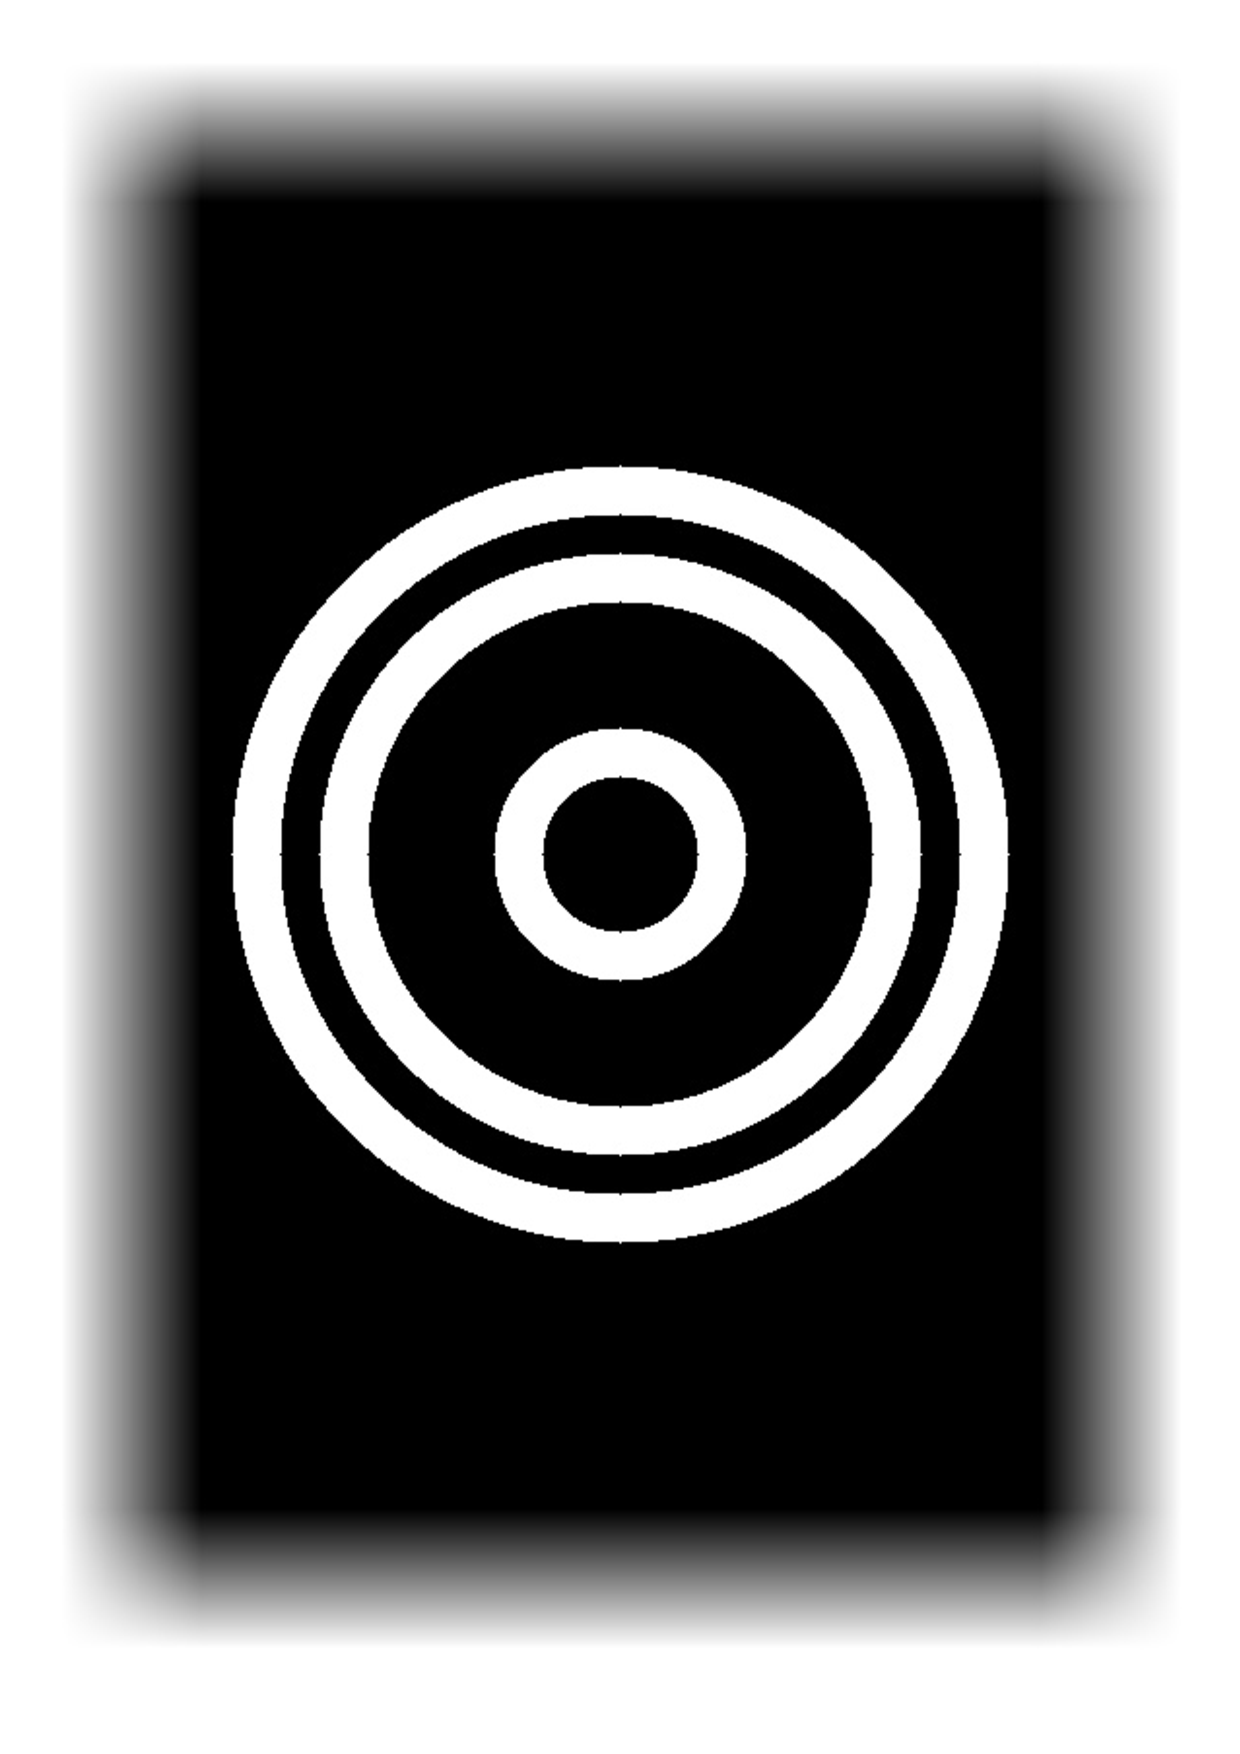
\includegraphics[width=.18\linewidth]{newconcentric_10.pdf}
  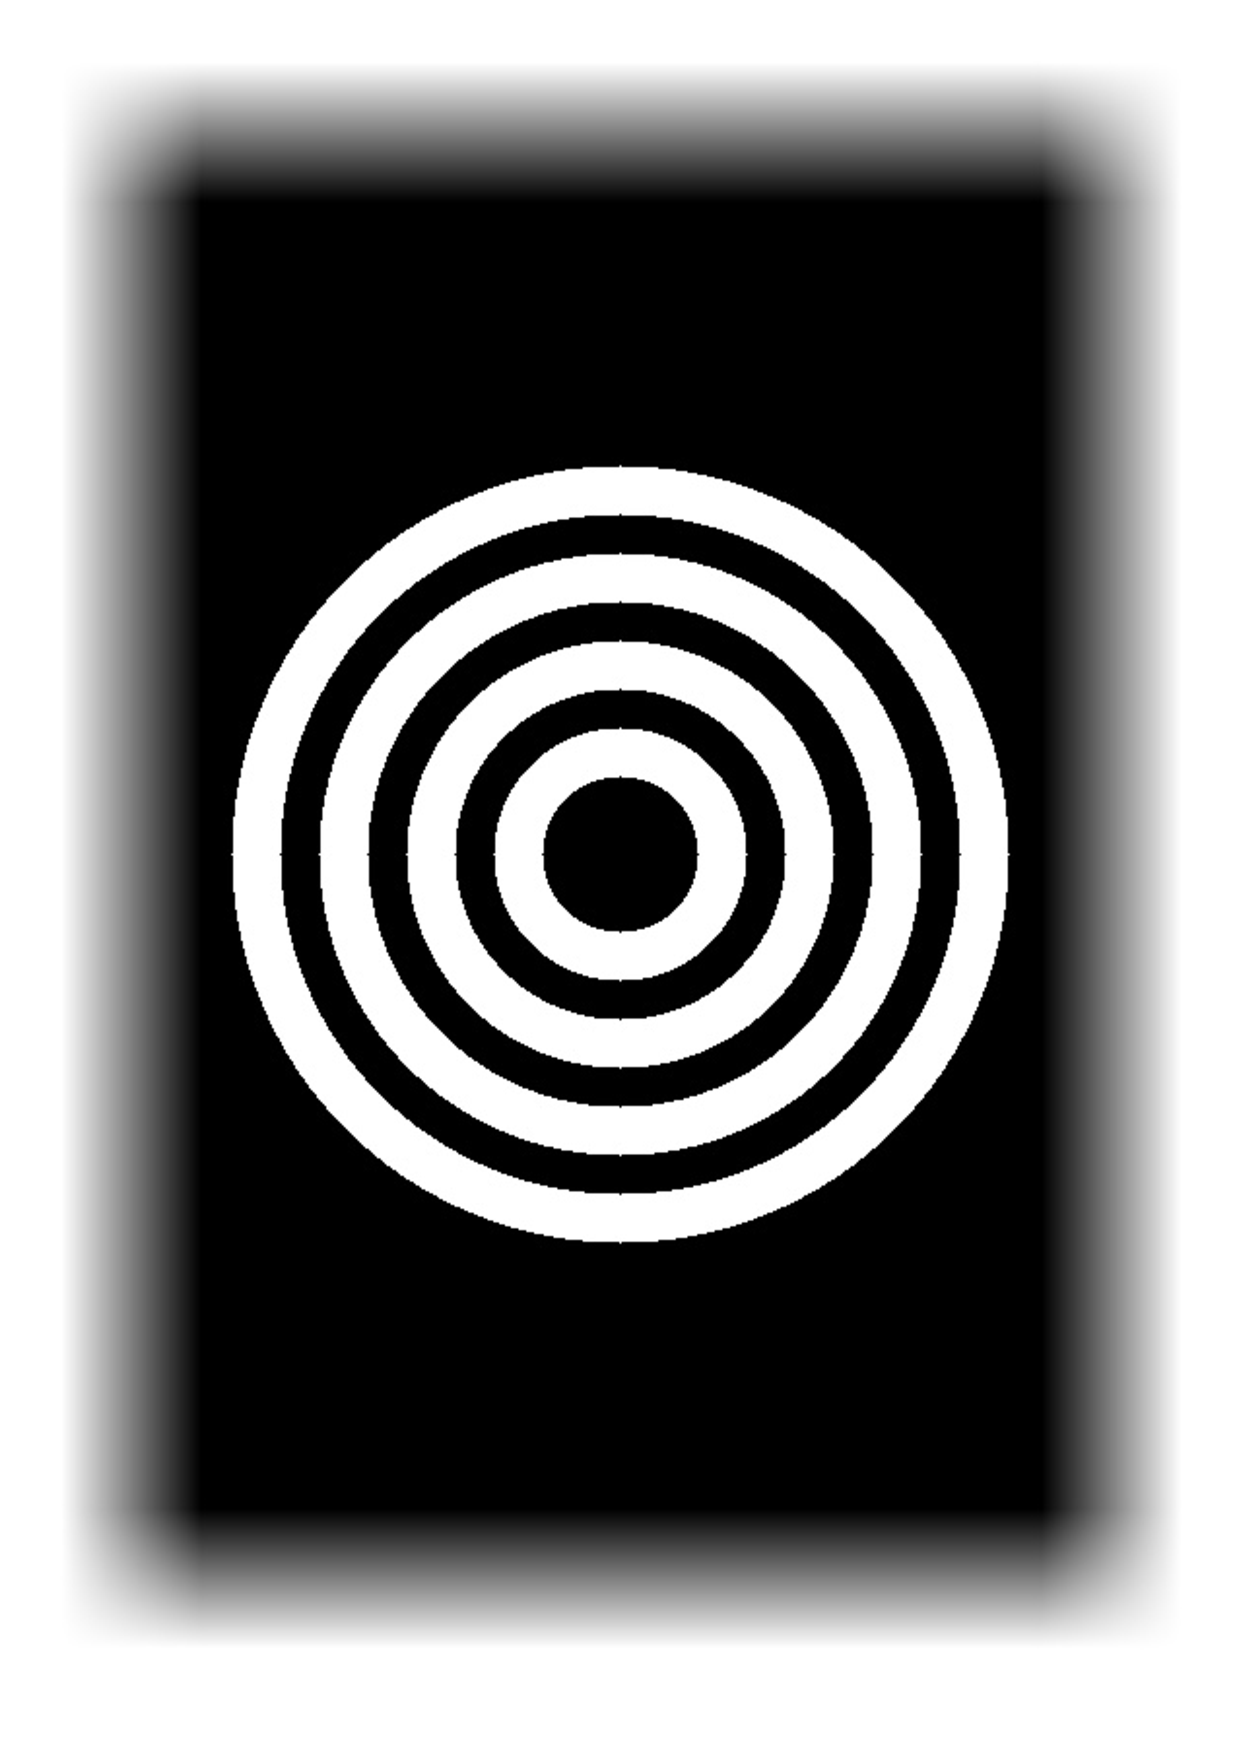
\includegraphics[width=.18\linewidth]{newconcentric_11.pdf}
  \caption{Two bit binary coded fiducials (from left to right: binary code 00,
  binary code 01, binary code 10, binary code 11.)}
  \label{fig:fiducials}
\end{figure}

Depending on which ring is present or absent, the resulting binary code will
change. The number of different patterns depends on the number of bits in the
binary code. For example, if the binary code has three bits, there will be a
maximum of three rings between marker-rings and we end up with eight
different patterns.  Figure \ref{fig:fiducials} shows a two bit binary coded
fiducials.

\subsection{Fiducial Detection Algorithm}

\begin{figure}
\centering
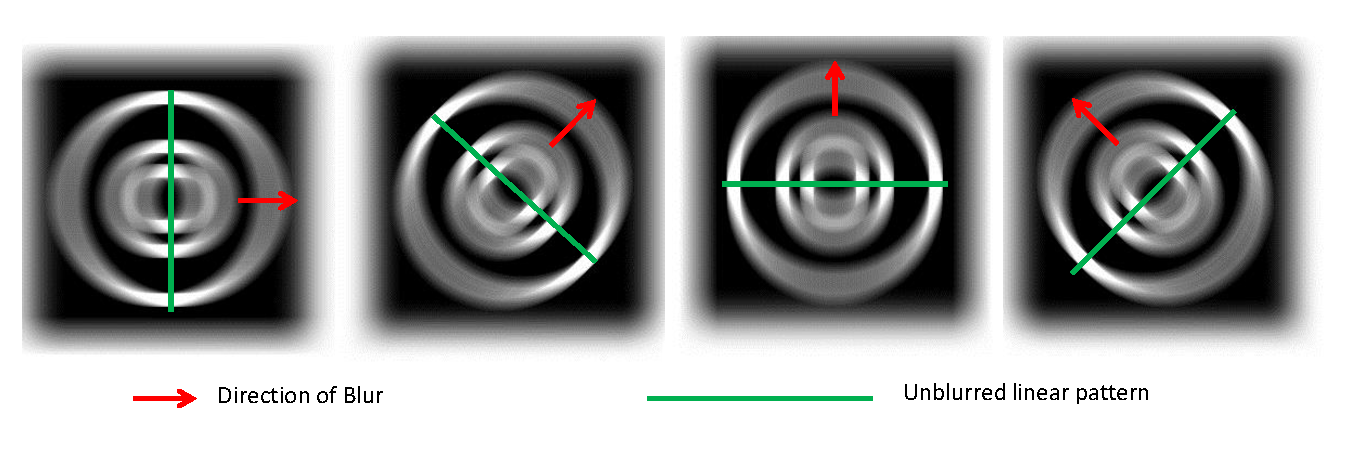
\includegraphics[width=0.8\linewidth]{blur_direction.pdf}
\caption{Figure showing how change in blur direction changes the location of
unblurred linear pattern.}
\label{fig:blur_direction}
\end{figure}

Our fiducial detection strategy is different from \cite{NaimarkF02,Pitag13} and works
under significant amounts of blur.   As previously mentioned, our approach works
under the observation that the motion blur for the quadcopter's camera
can be well modelled as linear motion.  This  linear motion blur assumption has
been shown to be reasonable in prior works targeting camera motion blur
(e.g.~\cite{Moshe:2003,Moshe:2004}). Under this assumption, the scene content
perpendicular to the blur direction is unaffected by the blur.  Because of our
circular design, the direction perpendicular to the linear motion will still be
recognizable as a linear pattern.  Figure \ref{fig:blur_direction} shows
examples of this using a pattern under various motion directions.

Figure \ref{fig:overall_flow} shows the process involved in fiducial
detection. We give a brief overview of our algorithm here with each step described 
in detail afterwards.  Our detection algorithm has four steps. Step 1,
we apply a Gabor filter on the image to isolate the
potential locations of the pattern.  Step 2, we find the clusters of patches
found in the Gabor output by clustering.  Step 3, performs Principal
Component Analysis (PCA) on each cluster to find the dominant direction
unaffected by blur.  Step 4, based on the direction we extract the intensity
profile of the pattern and classify the code using a K-Nearest Neighbor
classifier based on training data.

\begin{figure}[ht!]
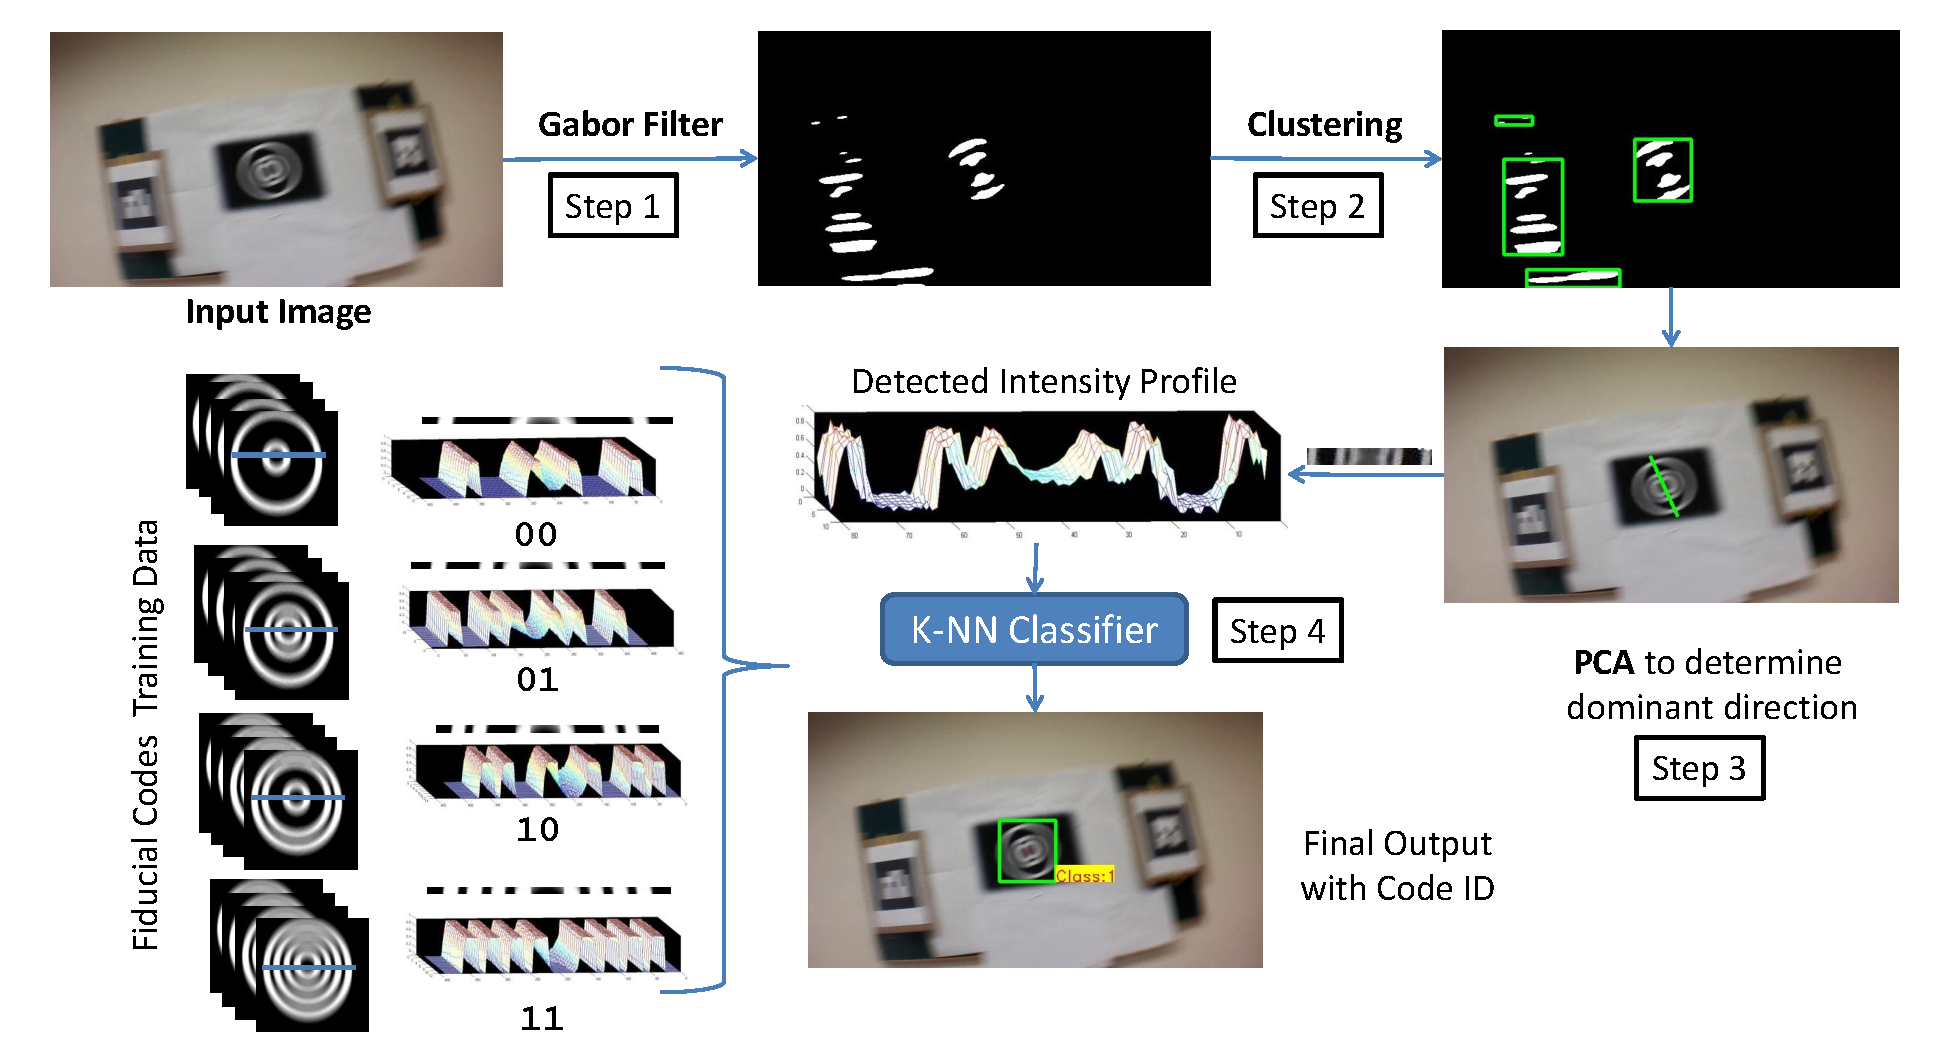
\includegraphics[width=\linewidth]{overall_flow.pdf}
\caption{An overview of our algorithm to detect and classify fiducial.
The four step process includes (Step 1) Gabor filtering,
(Step 2) component clustering, (Step 3) PCA to determine the dominant direction,
and (Step 4) K-NN classification using training-data captured for each pattern.}
\label{fig:overall_flow}
\end{figure}

\noindent Details of each of the steps are as follows:\\
\noindent\textbf{Gabor filter}~~A 2D Gabor filter is a Gaussian kernel function
modulated by a sinusoidal plane wave~\cite{Kruizinga:2002}. It is used to find
high gradient patches from the image. In our case, it is used to detect portions
of the circular fiducials that were not affected by the blur. 
We applied the Gabor filter in eight
different orientations ($\theta = 0, 45, 90, \ldots ,225, 270, 315$).  The
following parameters were used for creating each Gabor kernel: $\lambda$ (wavelength) $= 8$, $\gamma$
(aspect ratio) $= 0.5$, $\sigma$ (spread) $= 0.56\lambda$, $\psi$
(phase angle) $= 0$ (for real part), $\pi/2$ (for imaginary part).
Then $\ell^2$-norm of outputs along all orientations is calculated and finally
$\ell^2$-normalized image is thresholded with threshold set to $0.4$ (on scale of zero to
one).  For further details to the Gabor filter, see~\cite{Kruizinga:2002}.
%% MBS - is the Kruizinga filter resonable to cite?

\noindent\textbf{Clustering}~~The binarized Gabor filter responses are
treated as a set of connected components in the image.   Clustering
is used to find components that are located in a close spatial region.  We do
this via hierarchical clustering~\cite{ALGLIB} using unweighted
average linkage with a distance threshold set to 150.

\noindent\textbf{PCA}~~For each clustered set of components, we apply
PCA to determine the dominant direction.  This is done by examining the
orientation of the first principal component.  We then extract an intensity
profile patch in the input image along this direction as it extends through the
bounding box of the cluster. The signature of this profile will be used to
identify the code.

After finding the intensity profile, we examine it by
projecting the pixel intensities onto the PCA direction and record the
number and width of transitions.  If the number of transitions or the
width of the transitions is not consistent with what is allowable by
our code, we reject the clustered region as a potential fiducial.
Clustered components that have allowable transitions counts and transitions with
uniform widths are further considered for classification to determine
the binary code.

\noindent\textbf{Classification}~~As mentioned above, a small image patch
containing the intensity profile of the fiducial is used to identify the code.   We found
that a training-based method using K-NN gave better results than trying to
find binary code directly by determining the presence (or absence) of ring
at particular positions in the image patch. To build the training-data, a
synthetic fiducial pattern is blurred along 36 orientations (0, 10, 20, \ldots
, 350) with blur scale set to 40, and its intensity profile along the first
principal component from every output is taken as training data for that
fiducial pattern. Figure \ref{fig:training_data} shows the process of creating
training data for fiducial with binary code ``01'' embedded in it.  For an
input image patch, we normalize its intensity range and then compare it against
the training-data. The class label from the closest top $K=5$ images in the
training-data is used to label the patch.

\begin{figure}[h!]
\centering
  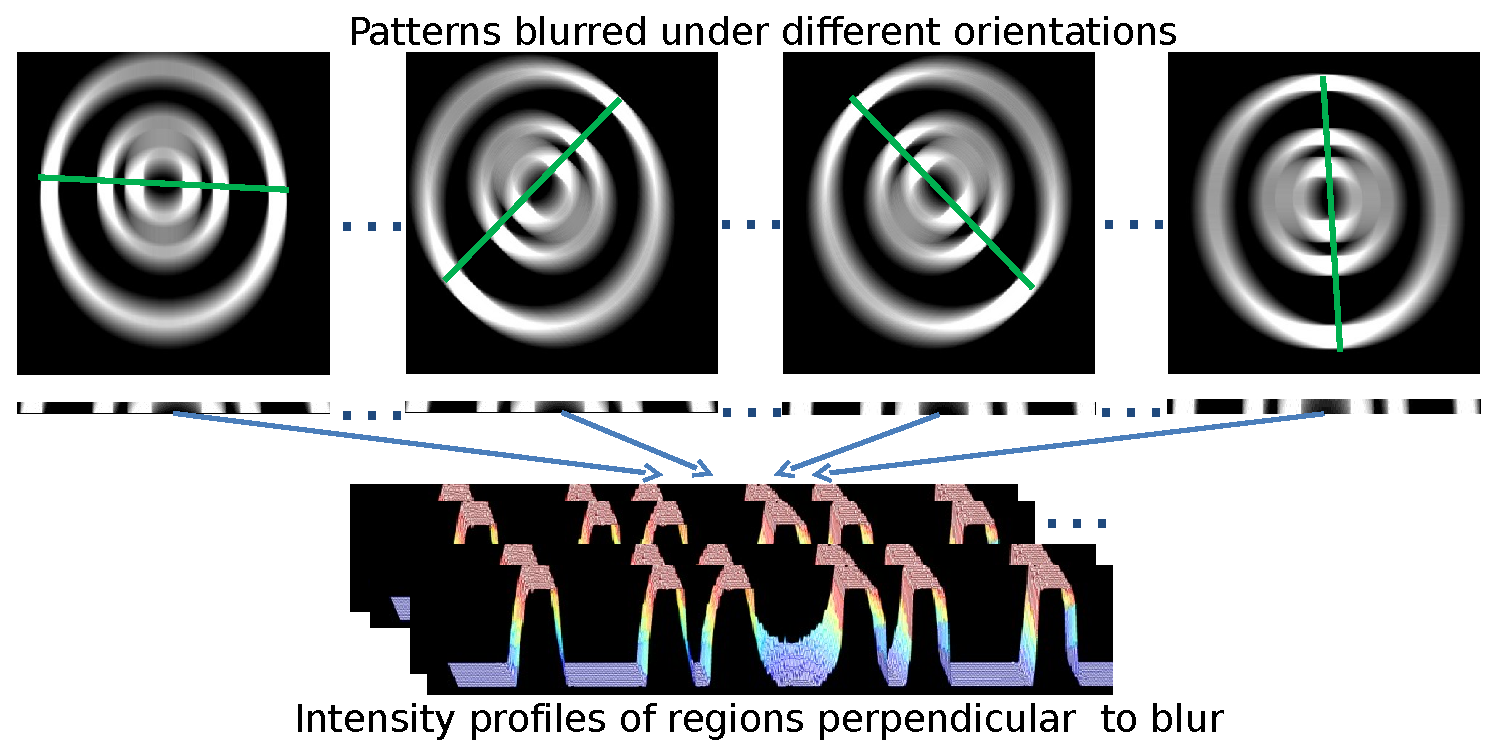
\includegraphics[width=0.8\linewidth]{training_data.pdf}
  \caption{Process to create training data for the fiducial pattern with binary
  code ``01''. The synthetic pattern is blurred along various orientations. Gabor
  filter is applied on the blurred pattern. Intensity profile is found along the
  first principal component of the clustered Gabor output. Same process is used
  to create training data for other fiducial patterns.}
  \label{fig:training_data}
\end{figure}

We are able to find the number of rings in the fiducial by finding
number of transitions in the intensity profile. To increase the classification
accuracy, training data for patterns having same number of rings are grouped together; e.g., in two bit
binary coded fiducial, training data for pattern ``01'' and ``10'' will be
grouped together. In three bit binary coded fiducial, training data for pattern
``001'', ``010'' and ``100'' will form one group, while training data for
pattern ``110'', ``011'' and ``101'' will be in other group, and so on. 
Depending on the number of detected rings in test pattern, it is matched
against corresponding group in the training data, again using  the K-NN. 
If we detect either zero rings or maximum possible
rings in the test pattern, there will be no need to do further classification, we
can classify the pattern as class 0 or the maximum class containing all 1s.

\section{Experimental Validation}

We have implemented our algorithm in C++ using the OpenCV library.
Experiments were performed on a PC with Intel Core i7 processor(@3.4GHz) and 4GB RAM.
Source code to generate and recognize the code, as well as the data sets used in
this paper will be made publicly available.  Video clips
of collected data are provided in the supplementary material.

Our system has been tested on several image sequences captured from an AR Drone
quadcopter.  The drone was flown indoors looking at patterns attached to
various walls. Each image sequence contains frames of different fiducial
patterns. Sample output for each fiducial pattern is shown in Figure
\ref{fig:out_outputs}-(a) -- Figure \ref{fig:out_outputs}-(d). Our detection
process takes around 0.3 seconds which translates to slightly over three frames per second.

Our system has also been tested on images containing multiple fiducial patterns
in the same frame. Our algorithm can successfully detected all fiducial patterns as
well as correctly classified them as shown in Figure \ref{fig:output_all}.

\begin{figure}[ht!]
\centering
  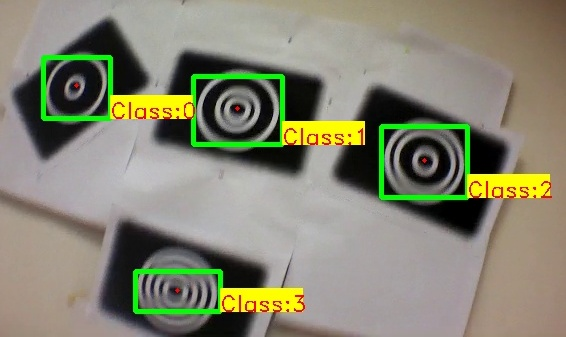
\includegraphics[width=.45\linewidth]{output_all_2.jpg}
  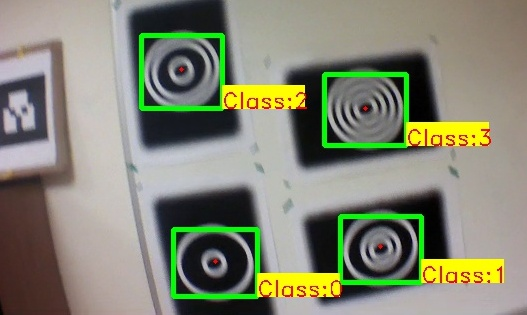
\includegraphics[width=.45\linewidth]{new_results/output_test_all1.jpg}
  \caption{Sample outputs containing all two bit binary coded fiducial patterns
  in single frame}
  \label{fig:output_all}
\end{figure}

\subsection{Comparisons}

We compare our results with the commonly used ARTag. We also compare
our results with Blur-driven tracker (BLUT)\cite{Wu:2011}.
\subsubsection{Comparison with ARTag}
First, we have repeated the blur simulation experiment on our fiducials as reported
in Section~\ref{sec:blurtest}.  Specifically, we build our blur resistant
patterns at 150$\times$150 pixel resolution and blurred them along various
orientations with different blur scales. Then, we tried to detect our fiducial using a 2-bit
patterns using algorithm presented in earlier section.

The comparison of recognition rate is shown in Figure
\ref{fig:simulated_blur}-(a). In this experiment, we use even more blur, up to 65
pixels. Figure \ref{fig:blur_maximum} shows the patterns under maximum blur they
can sustain are still be recognized. The graph in Figure
\ref{fig:simulated_blur}-(a) shows that our recognition is 100\% for all codes
except the ``00'' which is undetectable after 50 pixels blur (which is still
significantly better than ARTag).  Reasons for the ``00'' tags lower
performance is discussed in Section~\ref{sec:discussion}.

We also performed analysis to detect how accurately the center of the blur pattern 
can be localized under blur.  To do this, we have simulated data along different blur
orientations for all patterns over eight different blur scales (30 to 65 with
step size of 5). Values for the localization of the pattern ``00'' after blur
with 50 pixels is omitted since the pattern cannot be detected. From the Table in Figure
~\ref{fig:simulated_blur}-(b), it can be clearly seen that the mean error in
locating center by our algorithm is within approximate 3 pixels, or 3\% of the
diameter of fiducial.

\begin{figure}
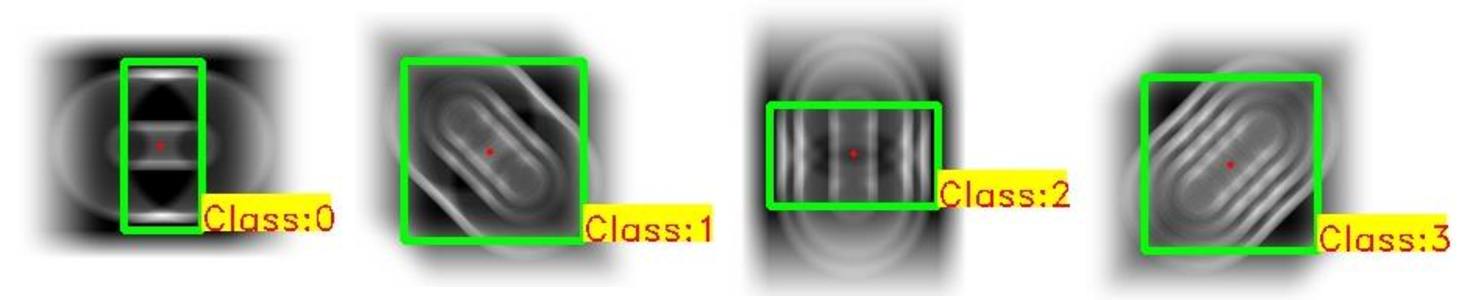
\includegraphics[width=\linewidth]{blur_maximum.pdf}
\caption{Result of our fiducial detection algorithm on blur simulated data.
Detection result is shown on each of our fiducial pattern, blurred at the
maximum scale it can handle.}
\label{fig:blur_maximum}
\end{figure}

\noindent\begin{figure}
\begin{tabular}{c|c}
\begin{subfigure}[b]{0.65\linewidth}
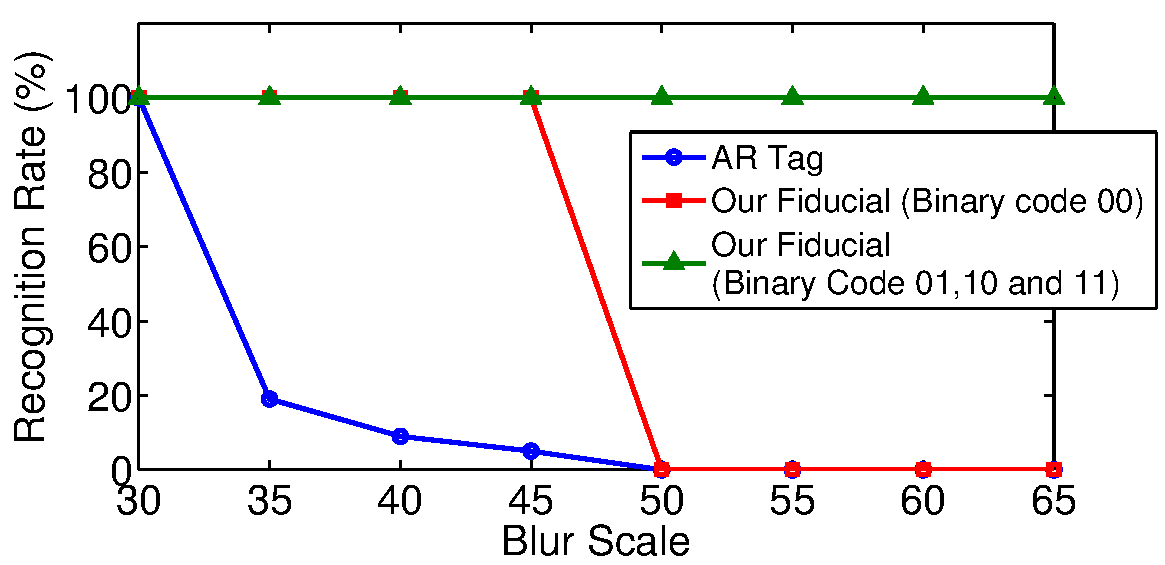
\includegraphics[width=\linewidth]{recognition_rate.pdf}
\caption{Comparison of recognition rate of fiducials}
\label{fig:recognition_rate}
\end{subfigure}
&
\begin{subfigure}[b]{0.33\linewidth}
\begin{tabularx}{\textwidth}{|c|Y|}
\cline{1-2}
\footnotesize{Blur} & \footnotesize{Mean($\pm$std) error}  \\
\footnotesize{angle} & \footnotesize{(in pixels)}  \\
\cline{1-2}
\footnotesize{0} & \footnotesize{1.33 $\pm$ 0.40}  \\
\footnotesize{22} & \footnotesize{2.42 $\pm$ 1.05} \\
\footnotesize{45} & \footnotesize{1.46 $\pm$ 0.65}  \\
\footnotesize{67} & \footnotesize{2.39 $\pm$ 1.28}  \\
\footnotesize{90} & \footnotesize{1.83 $\pm$ 0.25}  \\ 
\cline{1-2}
\end{tabularx}
\caption{Center localization error}
\label{tab:blur_angle_center}
\end{subfigure}
\end{tabular}
\caption{(a): Comparison of recognition rate of the ARTag and our fiducials on
blur simulated data at various blur scales. It can be seen that except for the
fiducial with binary code ``00'', our fiducial patterns are recognized all times.
(b): Table showing the mean error and standard deviation of the localized fiducial center
versus the ground truth.  Error is computed for various blur angles over
different blur scales.}
\label{fig:simulated_blur}
\end{figure}

We also compared results on the recorded feed using AR Drone quadcopter. In our
experimental setup, we have placed two ARTags in the scene along with our fiducial  to
compare the resilience of blur by each fiducial type. We have used
ar\_track\_alvar, ROS Wrapper for the ALVAR library~\cite{ros_alvar}, to detect
the ARTags from the stream captured with the quadcopter camera. In each test
dataset, we have used different two bit binary coded fiducial and recorded
video of around two minute duration (i.e., around 1000 frames).   The
quadcopter was flown in a routine manner in the room with its camera facing the
wall (see supplementary videos). The comparison of the recognition rate is
shown in Table \ref{tab:recongition_accuracy}. Recognition rate of our
fiducials ranges from 86.5\% to 94.1\%, while the ARTag is 60.3\% to 65.6\%.
Classification accuracy of all fiducials (ARTag as well as ours) was
approximately 100\%, i.e., when tags were detected they were the correct
fiducials and not other objects in the scene.

\begin{figure}[hb!]
\begin{subfigure}{\textwidth}
\centering
  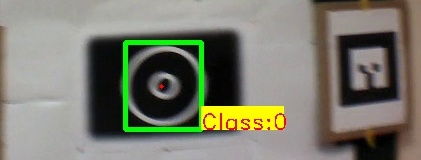
\includegraphics[width=0.4\linewidth]{output_00.jpg}
  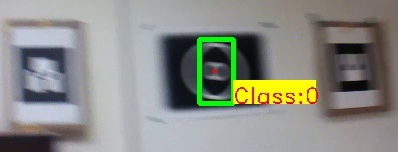
\includegraphics[width=0.4\linewidth]{new_results/output_00.jpg}
  \caption{Binary code ``00''}
  \label{fig:output0}
\end{subfigure}
\begin{subfigure}{\textwidth}
\centering
  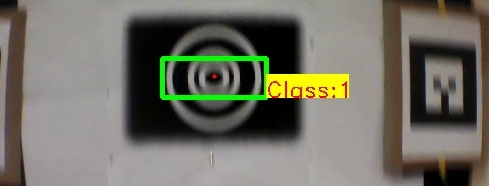
\includegraphics[width=0.4\linewidth]{output_01.jpg}
  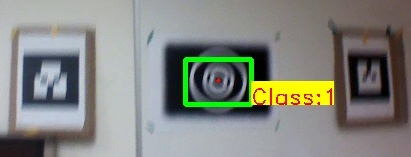
\includegraphics[width=0.4\linewidth]{new_results/output_01.jpg}
  \caption{Binary code ``01''}
  \label{fig:output1}
\end{subfigure}
\begin{subfigure}{\textwidth}
\centering
  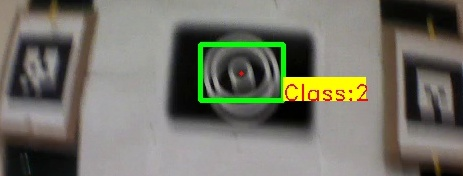
\includegraphics[width=0.4\linewidth]{output_10.jpg}
  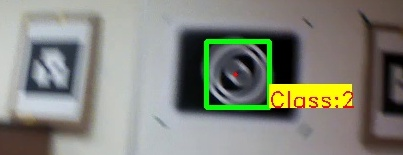
\includegraphics[width=0.4\linewidth]{new_results/output_10.jpg}
  \caption{Binary code ``10''}
  \label{fig:output2}
\end{subfigure}
\begin{subfigure}{\textwidth}
\centering
  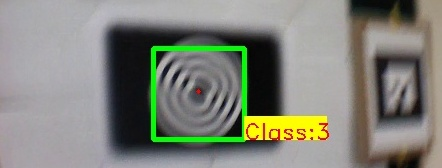
\includegraphics[width=0.4\linewidth]{output_11.jpg}
  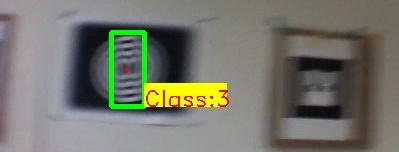
\includegraphics[width=0.4\linewidth]{new_results/output_11.jpg}
  \caption{Binary code ``11''}
  \label{fig:output3}
  \end{subfigure}
  \caption{Sample outputs for two bit binary coded fiducials on different
  datasets. Class label attached to the detected fiducial is decimal equivalent
  of the binary code embedded in the detected fiducial.}
  \label{fig:out_outputs}
\end{figure}

\begin{table}[h!]
\caption{Comparison of recognition rate of ARTag and our fiducials on real
data captured through AR Drone. Each row shows analysis of a test
dataset captured for our fiducial with different binary code embedded in it.
Each dataset has around 1000 frames captured representing roughly two minutes of video each.}
\centering
\begin{tabularx}{\textwidth}{|c|Y|Y|Y|Y|}
\cline{1-5}
\multirow{2}{*}{Test \#} & \multirow{2}{*}{Number of Frames}
&\multirow{2}{*}{Binary Code} &\multicolumn{2}{c|}{Recognition Rate (\%)} \\
\cline{4-5} & & & ARTag & Our Fiducial \\\cline{1-5}
1 & 1205 & 00 &  65.6 & 86.5  \\ \cline{1-5}
2 & 1047 & 01 &  61.9 & 94.1  \\ \cline{1-5}
3 & 1102 & 10 &  62.4 & 92.74 \\ \cline{1-5}
4 & 1081 & 11 &  60.3 & 93.54  \\ \cline{1-5}
\end{tabularx}
\label{tab:recongition_accuracy}
\end{table}

\subsubsection{Comparison with BLUT}

We also compare our approach with tracking designed for blurred input scenes.
We have used four image sequences (consisting of around 1000 frames each), each
one containing a different blur resistant fiducial pattern to test the performance of
BLUT \cite{Wu:2011} and compare it with our result on the same image sequence.
From the images in the top rows of Figure
\ref{fig:BLUT_compare_00}-\ref{fig:BLUT_compare_11}, we can see that BLUT is
able to track the fiducial when the position of fiducial does not change too
much in successive frames. Also, it can be seen that once BLUT looses 
track of the fiducial, it is not able to recover. Since our approach detects the
code in each frame, large changes in the patterns position is not an issue.
Our detection results are also shown in Figure
\ref{fig:BLUT_compare_00}-\ref{fig:BLUT_compare_11}.

We have also found that even if we reset the BLUT tracker after loosing track,
it will loose track again after around 100 frames, that is approximately within
6 seconds. When we checked the timestamp data from image header captured through
the AR Drone, we found that, there was a difference of 0.14 seconds between two
successive frames in the earlier case, which clearly indicates the dropping of
video frame (e.g., normal 30fps should be 0.033 seconds). Also, there were around 50
instances in 1000 frames where the timestamp difference between two successive
frames was greater than 0.1 seconds. As such, it appears one of the main
culprits causing the BLUT tracker to fail is the dropping of frames combined
with unstable motion of quadcopter resulting in large discrepancies in the
patterns position between successive frames.

\begin{figure}
\begin{subfigure}[b]{.19\textwidth}
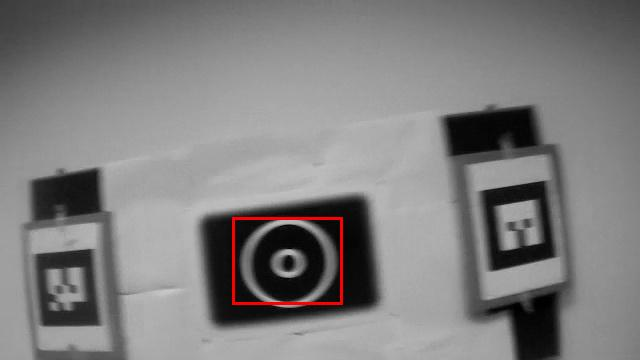
\includegraphics[width=\linewidth]{BLUT_output_00/2.jpg}
\end{subfigure}
\begin{subfigure}[b]{.19\textwidth}
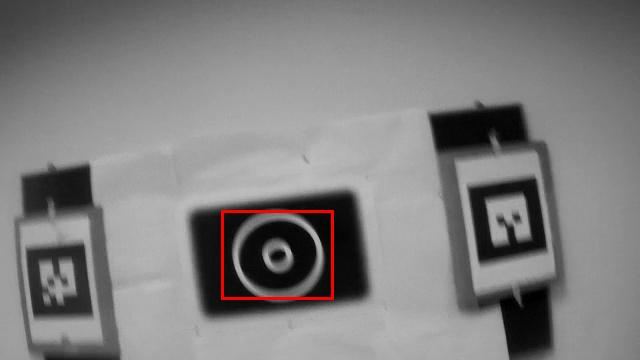
\includegraphics[width=\linewidth]{BLUT_output_00/3.jpg}
\end{subfigure}
\begin{subfigure}[b]{.19\textwidth}
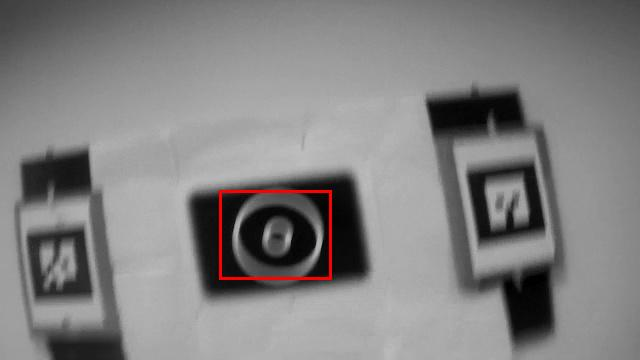
\includegraphics[width=\linewidth]{BLUT_output_00/4.jpg}
\end{subfigure}
\begin{subfigure}[b]{.19\textwidth}
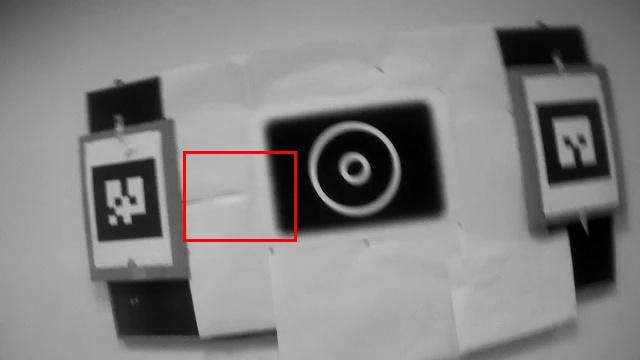
\includegraphics[width=\linewidth]{BLUT_output_00/5.jpg}
\end{subfigure}
\begin{subfigure}[b]{.19\textwidth}
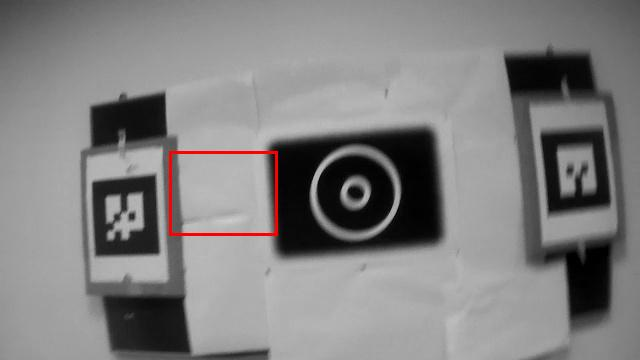
\includegraphics[width=\linewidth]{BLUT_output_00/6.jpg}
\end{subfigure}\\
\begin{subfigure}[b]{.19\textwidth}
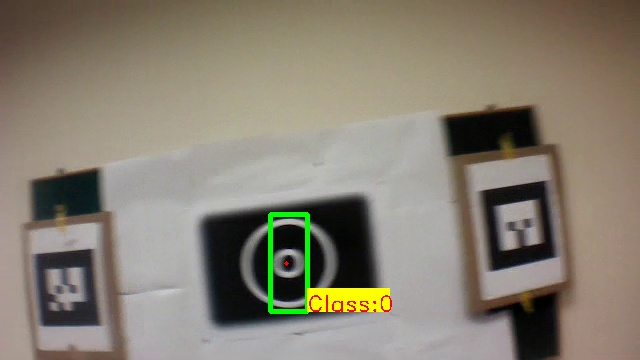
\includegraphics[width=\linewidth]{BLUT_input_00/output2.jpg}
\end{subfigure}
\begin{subfigure}[b]{.19\textwidth}
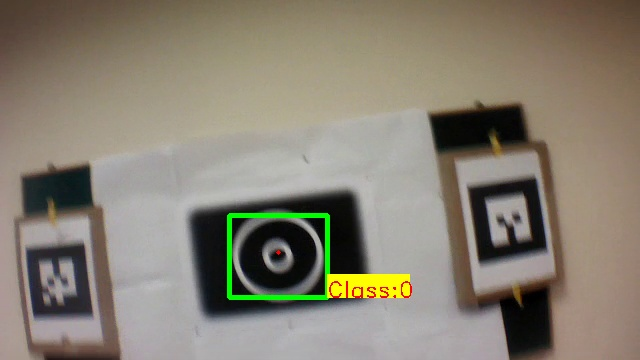
\includegraphics[width=\linewidth]{BLUT_input_00/output3.jpg}
\end{subfigure}
\begin{subfigure}[b]{.19\textwidth}
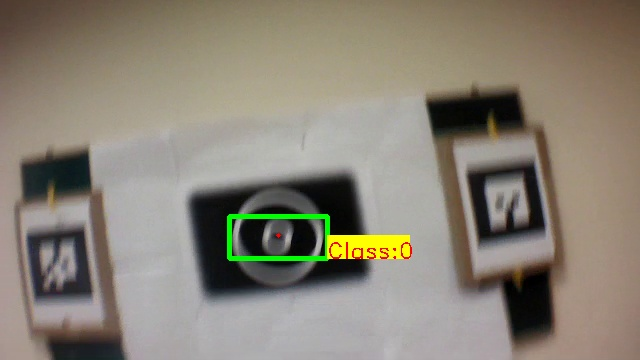
\includegraphics[width=\linewidth]{BLUT_input_00/output4.jpg}
\end{subfigure}
\begin{subfigure}[b]{.19\textwidth}
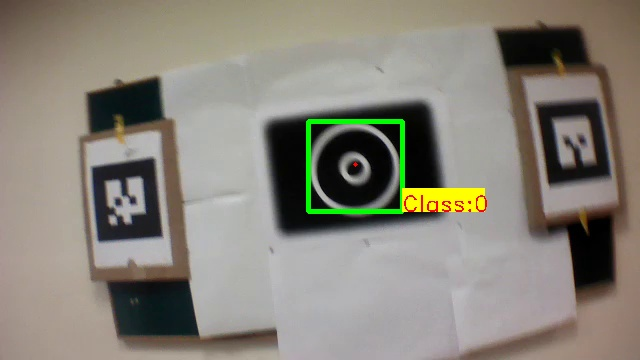
\includegraphics[width=\linewidth]{BLUT_input_00/output5.jpg}
\end{subfigure}
\begin{subfigure}[b]{.19\textwidth}
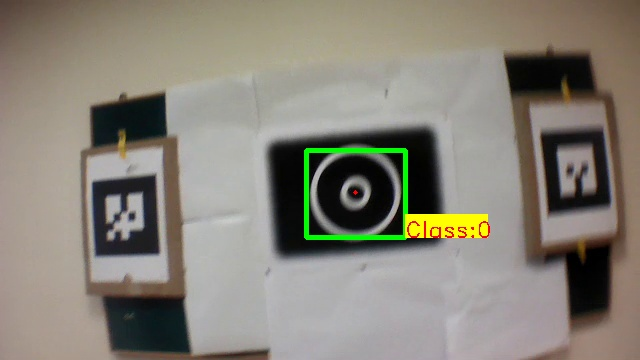
\includegraphics[width=\linewidth]{BLUT_input_00/output6.jpg}
\end{subfigure}
\caption{Top: Output of BLUT~\cite{Wu:2011} on sample image sequence containing ``00''
binary coded fiducial. Bottom: Output of our algorithm on the same image
sequence. BLUT is able to track the fiducial till the third frame, but from fourth
frame BLUT looses track of the fiducial. In first three frames, the size of the
fiducials is less but in fourth and fifth frame it is bigger, hinting at a sudden
forward movement of quadcopter.}
\label{fig:BLUT_compare_00}
\end{figure}

\begin{figure}
\begin{subfigure}[b]{.19\textwidth}
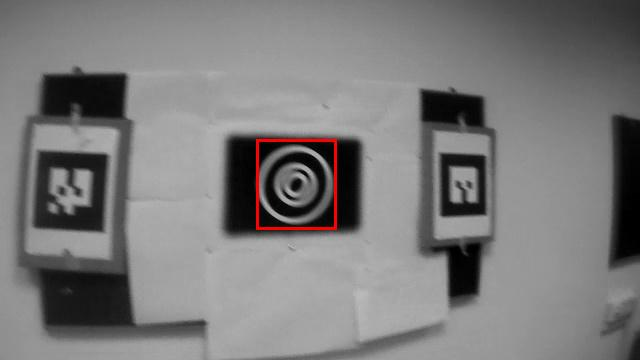
\includegraphics[width=\linewidth]{BLUT_output_01/11.jpg}
\end{subfigure}
\begin{subfigure}[b]{.19\textwidth}
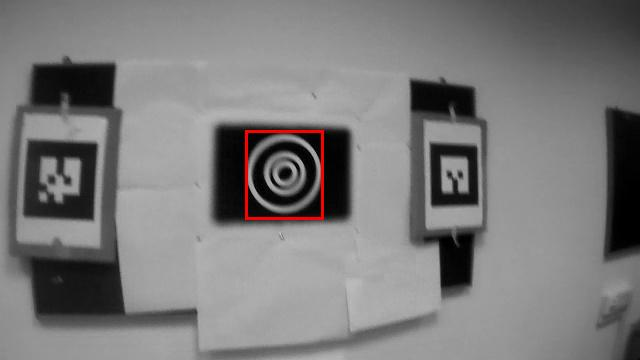
\includegraphics[width=\linewidth]{BLUT_output_01/12.jpg}
\end{subfigure}
\begin{subfigure}[b]{.19\textwidth}
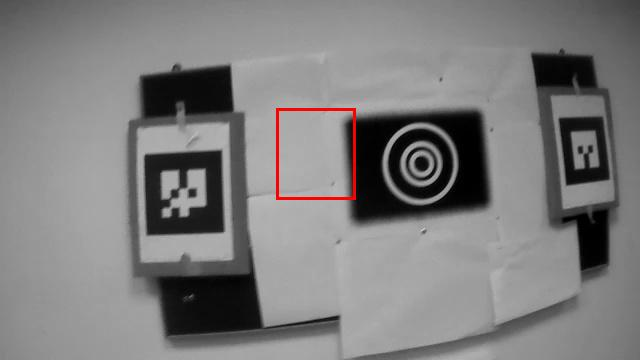
\includegraphics[width=\linewidth]{BLUT_output_01/13.jpg}
\end{subfigure}
\begin{subfigure}[b]{.19\textwidth}
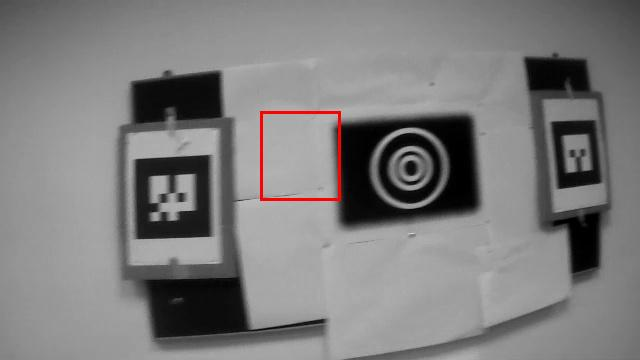
\includegraphics[width=\linewidth]{BLUT_output_01/14.jpg}
\end{subfigure}
\begin{subfigure}[b]{.19\textwidth}
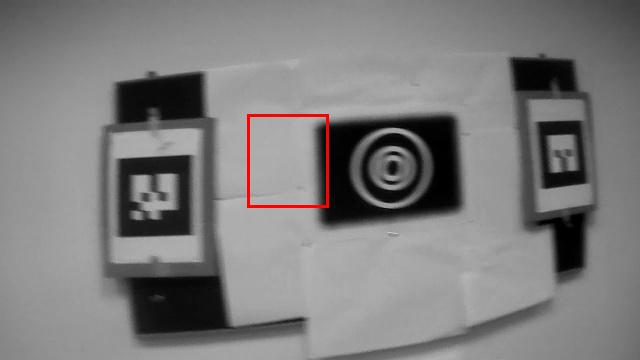
\includegraphics[width=\linewidth]{BLUT_output_01/15.jpg}
\end{subfigure}\\
\begin{subfigure}[b]{.19\textwidth}
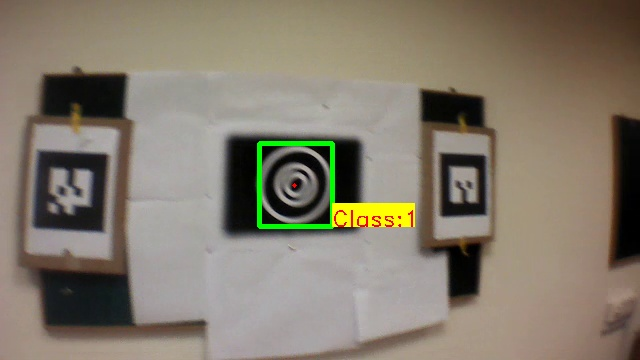
\includegraphics[width=\linewidth]{BLUT_input_01/output11.jpg}
\end{subfigure}
\begin{subfigure}[b]{.19\textwidth}
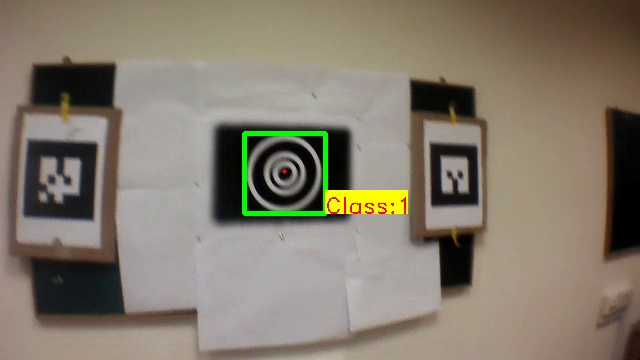
\includegraphics[width=\linewidth]{BLUT_input_01/output12.jpg}
\end{subfigure}
\begin{subfigure}[b]{.19\textwidth}
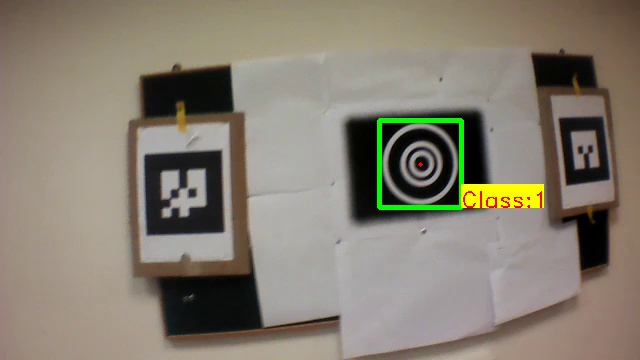
\includegraphics[width=\linewidth]{BLUT_input_01/output13.jpg}
\end{subfigure}
\begin{subfigure}[b]{.19\textwidth}
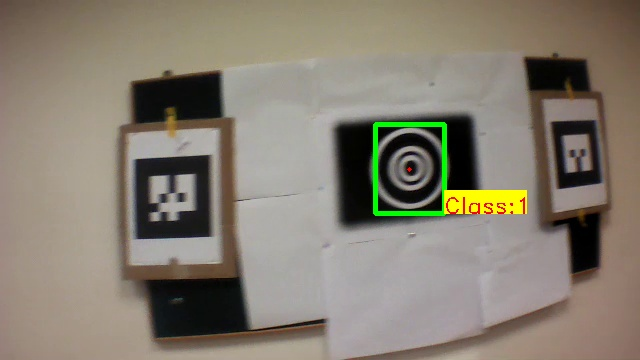
\includegraphics[width=\linewidth]{BLUT_input_01/output14.jpg}
\end{subfigure}
\begin{subfigure}[b]{.19\textwidth}
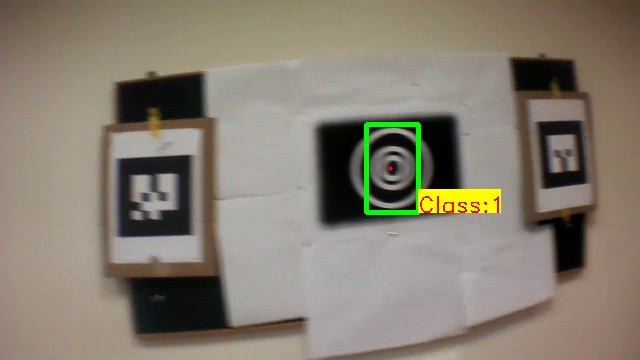
\includegraphics[width=\linewidth]{BLUT_input_01/output15.jpg}
\end{subfigure}
\caption{Top: Output of BLUT~\cite{Wu:2011} on sample image sequence containing
``01'' binary coded fiducial. Bottom: Output of our algorithm on the same image
sequence. BLUT looses the track from the third frame.}
\label{fig:BLUT_compare_01}
\end{figure}

\begin{figure}
\begin{subfigure}[b]{.19\textwidth}
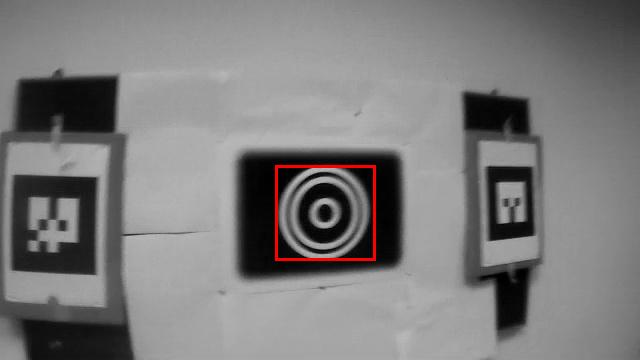
\includegraphics[width=\linewidth]{BLUT_output_10/1.jpg}
\end{subfigure}
\begin{subfigure}[b]{.19\textwidth}
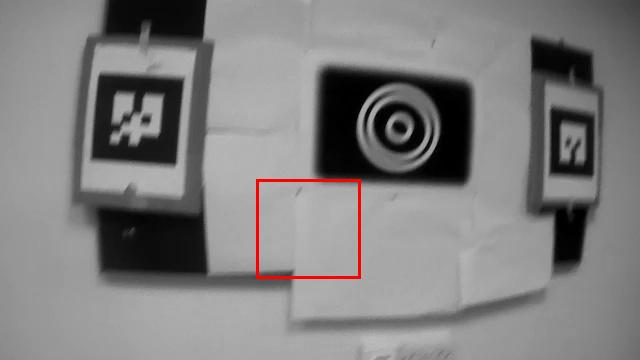
\includegraphics[width=\linewidth]{BLUT_output_10/2.jpg}
\end{subfigure}
\begin{subfigure}[b]{.19\textwidth}
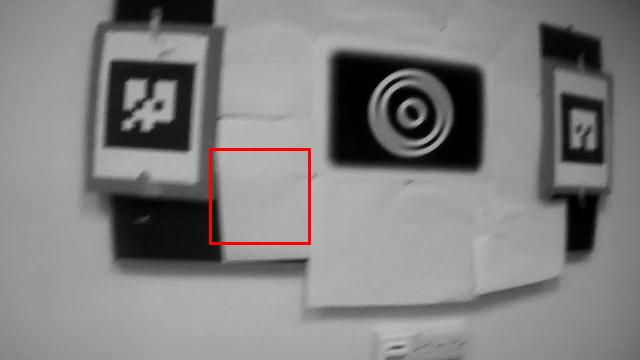
\includegraphics[width=\linewidth]{BLUT_output_10/3.jpg}
\end{subfigure}
\begin{subfigure}[b]{.19\textwidth}
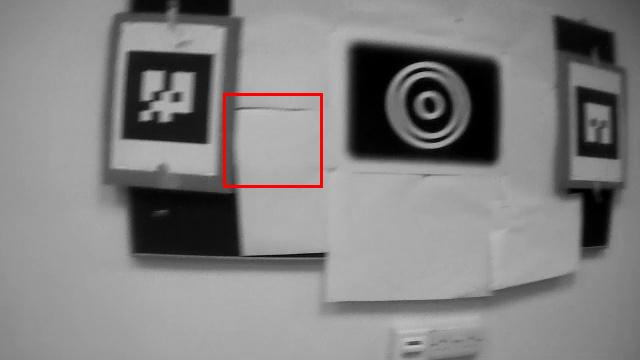
\includegraphics[width=\linewidth]{BLUT_output_10/4.jpg}
\end{subfigure}
\begin{subfigure}[b]{.19\textwidth}
\includegraphics[width=\linewidth]{BLUT_output_10/5.jpg}
\end{subfigure}\\
\begin{subfigure}[b]{.19\textwidth}
\includegraphics[width=\linewidth]{BLUT_input_10/output1.jpg}
\end{subfigure}
\begin{subfigure}[b]{.19\textwidth}
\includegraphics[width=\linewidth]{BLUT_input_10/output2.jpg}
\end{subfigure}
\begin{subfigure}[b]{.19\textwidth}
\includegraphics[width=\linewidth]{BLUT_input_10/output3.jpg}
\end{subfigure}
\begin{subfigure}[b]{.19\textwidth}
\includegraphics[width=\linewidth]{BLUT_input_10/output4.jpg}
\end{subfigure}
\begin{subfigure}[b]{.19\textwidth}
\includegraphics[width=\linewidth]{BLUT_input_10/output5.jpg}
\end{subfigure}
\caption{Top: Output of BLUT~\cite{Wu:2011} on sample image sequence containing
``10'' binary coded fiducial. Bottom: Output of our algorithm on the same image
sequence. From the second frame, BLUT looses track.}
\label{fig:BLUT_compare_10}
\end{figure}

\begin{figure}
\begin{subfigure}[b]{.19\textwidth}
\includegraphics[width=\linewidth]{BLUT_output_11/2.jpg}
\end{subfigure}
\begin{subfigure}[b]{.19\textwidth}
\includegraphics[width=\linewidth]{BLUT_output_11/3.jpg}
\end{subfigure}
\begin{subfigure}[b]{.19\textwidth}
\includegraphics[width=\linewidth]{BLUT_output_11/4.jpg}
\end{subfigure}
\begin{subfigure}[b]{.19\textwidth}
\includegraphics[width=\linewidth]{BLUT_output_11/5.jpg}
\end{subfigure}
\begin{subfigure}[b]{.19\textwidth}
\includegraphics[width=\linewidth]{BLUT_output_11/6.jpg}
\end{subfigure}\\
\begin{subfigure}[b]{.19\textwidth}
\includegraphics[width=\linewidth]{BLUT_input_11/output2.jpg}
\end{subfigure}
\begin{subfigure}[b]{.19\textwidth}
\includegraphics[width=\linewidth]{BLUT_input_11/output3.jpg}
\end{subfigure}
\begin{subfigure}[b]{.19\textwidth}
\includegraphics[width=\linewidth]{BLUT_input_11/output4.jpg}
\end{subfigure}
\begin{subfigure}[b]{.19\textwidth}
\includegraphics[width=\linewidth]{BLUT_input_11/output5.jpg}
\end{subfigure}
\begin{subfigure}[b]{.19\textwidth}
\includegraphics[width=\linewidth]{BLUT_input_11/output6.jpg}
\end{subfigure}
\caption{Top: Output of BLUT~\cite{Wu:2011} on sample image sequence containing
``11'' binary coded fiducial. Bottom: Output of our algorithm on the same image
sequence. BLUT lost the track from third frame. There is sudden reversal of
direction from the quadcopter in the third frame. In first two frames, the quadcopter was
going up, but suddenly moved down.}
\label{fig:BLUT_compare_11}
\end{figure}

\section{Discussion}\label{sec:discussion}

We have demonstrated the effectiveness of our blur invariant fiducial both
synthetically and on real video clips captured from a quadcopter.   Our approach obtains
approximately 86-95\% recognition rate on fiducals in real scenes compared to existing codes
that are around 64\%.  We discuss some limitations of our approach in the following.

\noindent\textbf{Processing Time}~~Currently, our processing time (0.3 seconds
per frame) does not provide real-time performance.  As such, we currently
envision this will be used in an offline manner for performing analysis of
flight paths. Code profiling revealed that the Gabor filtering along the eight
directions takes most of the time (0.03 -- 0.04 seconds per orientation).  Either an
improved Gabor filter scheme is required or an alternative strategy for
detection is required.

\noindent\textbf{False Negatives}~~We found that sometimes our detection
algorithm fails to recognize our fiducial with binary code ``00'' when there is
large amount of blur.  The is because when there is too much blur, the innermost
ring's response in the Gabor output is too low and not detected properly.
This problem can be resolved by increasing the radius of innermost ring to
reduce the effect of blur on the innermost ring. 

\noindent\textbf{Pose Estimation}~~We note that other markers are able to give
full pose estimation after detection.  However, we are only able to reliably detect
the center point and therefore cannot estimate pose.  Of course, if four
markers were used in a known order, pose could be estimated. The current
resolution of onboard camera will be main hurdle to clear before we can
effectively use multiple markers in each scene.

\noindent\textbf{Number of Fiducials}~~Currently, compared to ARTag fiducial
markers, we are able to generate less number of fiducials. Many applications in
robotics (e.g. quadcopter navigation) may not require large number of fiducial
markers as available by ARTag.  Most of the time, it is sufficient to have 4-6
different fiducial patterns. Still, we may be able to generate a larger number of
fiducials by using color backgrounds. This is an area interest for further
investigation.

\section{Conclusion}

Quadcopters are subject to quick and unstable motions that can cause significant
motion blur in the captured images. This severely affects the detection rate of
existing fiducial markers. We proposed the design of a fiducial that is
resistant to motion blur. Our design of contrasting concentric rings is based on the
observation that the direction perpendicular to the motion blur direction will
be unaffected by the blur and therefore still be recognizable. We have shown
through experimental validation that our fiducial will work under large
amounts of motion blur and can significantly outperform existing fiducial
markers under this scenario.

{\small
\bibliographystyle{ieee}
\bibliography{egbib}
}
\end{document}
